\section{Spectraèdres réels}

\newcommand\ssp{symétrique semi-définie positive}
\newcommand\ssps{symétriques semi-définies positives}
\newcommand\Ssp{Symétrique semi-définie positive}
\newcommand\Ssps{Symétriques semi-définies positives}

\subsection{définiion?}
\todo{trouver un nom}

\begin{definition}
	On appelle \emph{matrice symétrique semi-définie positive} toute matrice réelle symétriques et à valeurs propres positives ou nulles.
	On notera $\mathcal{S}_n^+\left(\mathbb{R}\right) $ l'ensemble de telles matrices et $M \succeq 0$ le fait que $M \in \mathcal{S}_n^+\left(\mathbb{R}\right)$.
\end{definition}

\begin{remarque}
	On remarquera que demander la symétrie, n'est, dans le cas réel, qu'un moyen de s'assurer d'obtenir des valeurs propres réelles grâce au théorème spectral.
\end{remarque}
\begin{propriete}
	L'ensemble $\mathcal{S}_n^+\left( \mathbb{R} \right) $ est un cône convexe fermé.
\end{propriete}

\begin{definition}
	On appelle \emph{spectraèdre} l'intersection de $\mathcal{S}_n^+\left(\mathbb{R}\right)$ avec un \simone{espace} affine $\mathcal{L}$ de $\mathcal{S}_n\left(\mathbb{R}\right)$.
\end{definition}

En écrivant l'hyperplan $\mathcal{L}$ de $\mathcal{S}_n^+\left(\mathbb{R}\right)$ sous sa forme paramétrique \textit{i.e.} comme l'ensemble des matrices de la forme $A_0 + x_1 A_1 + \ldots x_s A_s$ pour $A_0,\ldots, A_s$ des matrices symétriques fixées on peut définir le spéctraèdre $\mathcal{S} = \mathcal{L} \cap \mathcal{S}_n^+\left(\mathbb{R}\right)$ comme
\simone{$\mathcal{S} = \{A := A_0 + x_1A_1 + \ldots + x_s A_s | A \succeq 0, (x_1,\ldots,x_s) \in \mathbb{R}^s\}$}. On identifie alors souvent ce dernier à sa préimage dans $\mathbb{R}^s$
$S = \{(x_1,\ldots,x_s) \simone{\in \mathbb{R}^s} | A_0+ x_1A_1 + \ldots+ x_s A_s \succeq 0 \}. $
\todo{image + exemple}

\simone{
  \begin{ex} Un exemple celèbre de spectraèdre est l'ensemble des matrices symétrique semi-définie positives
    avec diagonale $(1,1,1)$:
    $$
    S = \left\{
    \begin{pmatrix} x_1 \\ x_2 \\ x_3 \end{pmatrix} \in \mathbb{R}^3 |
    A:=\begin{pmatrix} 1 & x_1 & x_2 \\ x_1 & 1 & x_3 \\ x_2 & x_3 & 1 \end{pmatrix} \succeq 0
    \right\}.
    $$
    La surface algébrique définie par $\det A(x_1,x_2,x_3) = 0$ est dite {\it cubique de Cayley} (Figure
    \Cref{cayley}).
    Les quatres points singuliers correspondent à quatre matrices semi-définies positives de rang 1.
    \begin{figure}[!ht]
      \label{cayley}
      \centering
      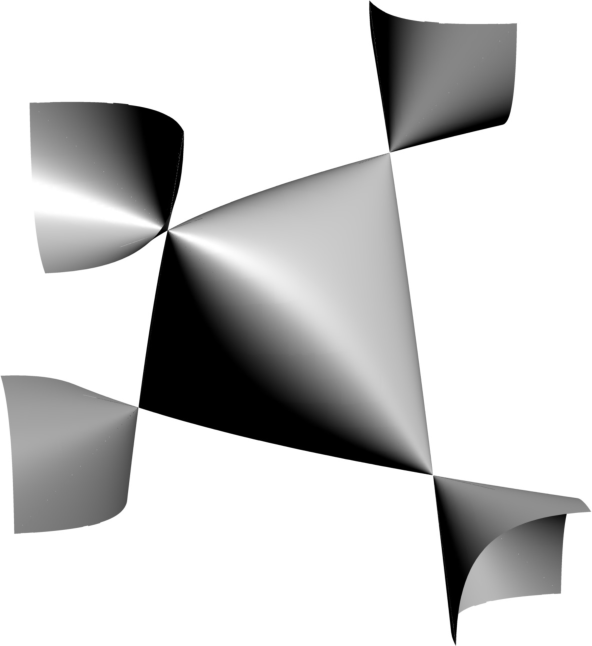
\includegraphics[scale=0.3]{figures/cayley.pdf}
      \caption{}
    \end{figure}
  \end{ex}
}

\subsection{Programmation semi-définie positive}

On appelle alors programmation semi-définie le problème d'optimisation consistant à minimiser une application linéaire sur un spéctraèdre que l'on formulera comme :
\begin{equation}
	\tag{PSD}
	\begin{matrix}
		\text{Minimiser } c.x \text{ tel que}\\
		A_0 + \sum \limits_{i=1}^s x_{i}A_{i} \succeq 0
	\end{matrix}
	\label{Psd} 
\end{equation}

pour $A_0,\ldots, A_s$ des matrices symétriques fixées et $c$ un vecteur représentant le coût.

Ce problème se résout en temps polynomial en la taille des matrices grâce à des techniques d'optimisation convexe. \todo{exemples}

Si à première vue ce problème peut sembler très spécifique il n'en est rien et de nombreux autres problèmes se rapportent à celui-ci.

Le premier exemple étant que 
